\chapter{Pattern Matching}\label{ch:pattern-matching}

\todo{
OCL (Object Constraint Language),
QVT (Query View Transform),
}

\section{Fulib-Tables}\label{sec:fulib-tables}

FulibTables\cite{fulibTables} ist eine Java-Bibliothek, mit der Objektstrukturen als Tabellen behandelt werden können.
Diese Tabellen dienen als Grundlage für einen Pattern Matcher, den die Bibliothek ebenfalls anbietet.
Im folgenden Abschnitt werden zunächst die Tabellen und deren Operationen anhang eines einfachen Beispiels vorgestellt.
Daraufhin werden die Möglichkeiten zum Pattern Matching betrachtet.

\subsection{Tabellen}\label{subsec:tables}

Um Tabellen nutzen zu können, wird zunächst ein Datenmodell benötigt.
Dazu soll beispielhaft ein Modell von einem fiktiven Spiel für mehrere Spieler verwendet werden.
Jeder Spieler hat ein oder mehrere Häuser, die eine Zahl von Einheiten haben.
Ziel des Spiel ist es, in mindestens einem Haus eine bestimmte Anzahl von Einheiten zu erreichen.
Das entsprechende Klassendiagramm ist in Abbildung~\ref{fig:game-class-diagram} zu sehen.

\begin{figure}
    \centering
    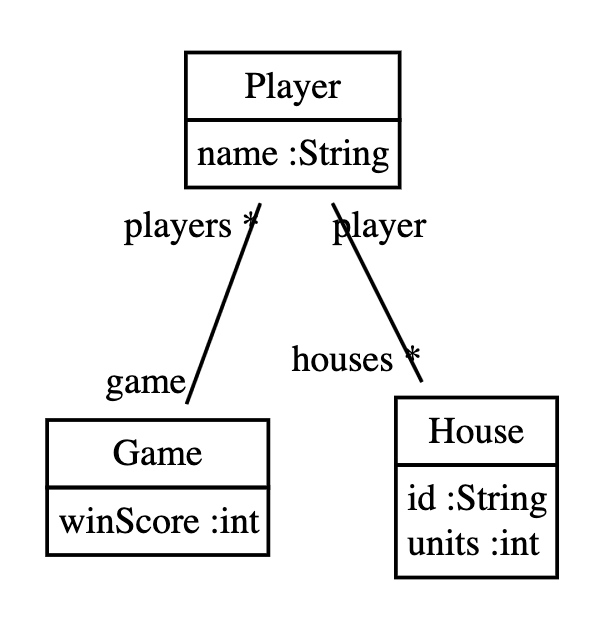
\includegraphics[width=0.4\textwidth]{chapter/pattern-matching/img/game-class-diagram.png}
    \caption{Beispiel-Klassendiagramm zur Verwendung von FulibTables}
    \label{fig:game-class-diagram}
\end{figure}

Es werden nun einige Beispielobjekte zu diesem Modell erstellt, die den Endzustand des Spiels beschreiben.

\begin{jcodeblock*}{breaklines}
    Game game = new Game().setWinScore(60);
    Player alice = new Player().setName("Alice").setGame(game);
    Player bob = new Player().setName("Bob").setGame(game);
    Player charlie = new Player().setName("Charlie").setGame(game);
    House a1 = new House().setId("a1").setUnits(30).setPlayer(alice);
    House a2 = new House().setId("a2").setUnits(20).setPlayer(alice);
    House b1 = new House().setId("b1").setUnits(40).setPlayer(bob);
    House c1 = new House().setId("c1").setUnits(60).setPlayer(charlie);
\end{jcodeblock*}

Das zugehörige Objektdiagramm ist in Abbildung~\ref{fig:game-object-diagram} zu sehen.

\begin{figure}
    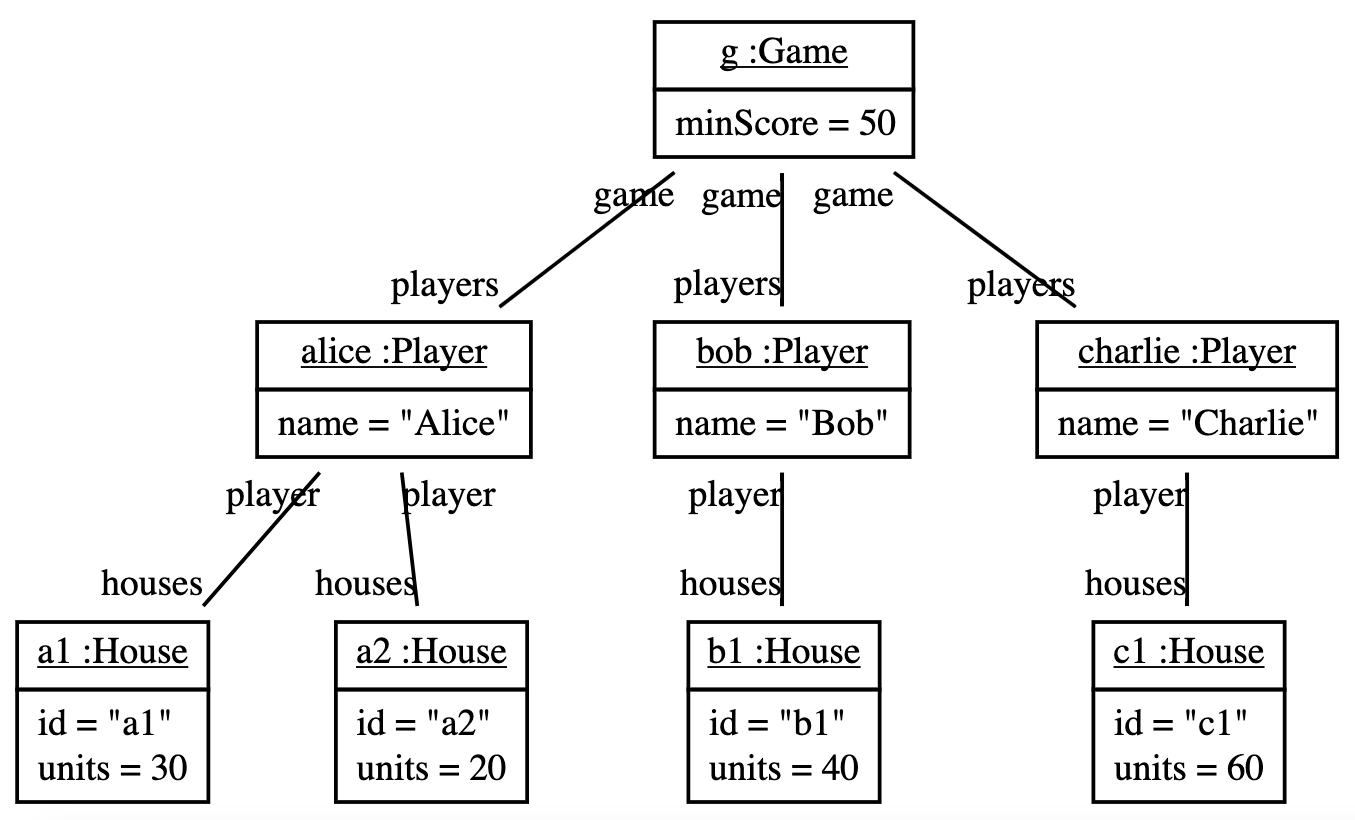
\includegraphics[width=\textwidth]{chapter/pattern-matching/img/game-object-diagram.png}
    \caption{Beispiel-Objektdiagramm zur Verwendung von FulibTables}
    \label{fig:game-object-diagram}
\end{figure}

Nun kann eine Tabelle angelegt werden.
In FulibTables besteht jede Tabelle aus mindestens einer Spalte und null oder mehr Zeilen\footnote{Der Spaltenname zählt dabei nicht als Zeile.}.
Tabellen können \emph{erweitert} oder \emph{eingeschränkt} werden, wobei Spalten entstehen oder entfernt werden.
Beim Erweitern entstehen neue Tabellen-Instanzen,
die sich die Daten der ursprünglichen Tabelle teilen.
Jede Tabellen-Instanz hat eine Spalte, auf die sie \emph{zeigt}.
Operationen auf der Tabelle beziehen sich i.d.R.\ auf diese Spalte,
wirken sich aber durch das geteilte Datenmodell auf alle anderen Instanzen aus.
Zunächst wird nur eine einfache Tabelle mit einer Spalte und einer Zeile benötigt.
Dafür müssen der Name der ersten Spalte sowie eine Liste von Objekten, die die Zeilen dieser Spalte bilden, angegeben werden.
Hier wird zunächst nur eine Zeile gebraucht.

\begin{jcodeblock}
    ObjectTable<Game> games = new ObjectTable<>("Games", game);
\end{jcodeblock}

Diese lässt sich wie folgt darstellen:

\begin{tabular}{|c|}
    \hline
    \textbf{Games} \\
    \hline
    g \\
    \hline
\end{tabular}

Auf dieser Tabelle lässt sich nun eine Erweiterung durchführen, was mit der Methode \code{expand} erreicht wird.
Diese erwartet zuerst einen Namen für die neue Spalte, die sowohl der alten Tabelle hinzugefügt wird als auch Ziel der neuen Tabellen-Instanz ist.
Weiterhin wird eine Funktion in Form eines Lambda-Ausdrucks übergeben.
Dieser wird für jede Zeile der Tabelle aufgerufen.
Die Ergebnisse bilden dann die Zeilen der neuen Spalte.
Dies wird anhand des Beispiels deutlich:

\begin{jcodeblock*}{breaklines,escapeinside=||}
    Table<Integer> winScores = games.expand("Win Scores", Game::getWinScore|\footnotemark|);
\end{jcodeblock*}
\footnotetext{Bei diesem Ausdruck handelt es sich um eine Methodenreferenz, die zu dem Lambda-Ausdruck \jcode{game -> game.getWinScore()} äquivalent ist.}

Die neue Tabelle lässt sich wie folgt darstellen:

\begin{tabular}{|c|c|}
    \hline
    \textbf{Games} & \textbf{Win Scores} \\
    \hline
    g & 60 \\
    \hline
\end{tabular}

Die \code{expand}-Methode ist geeignet für Attribute und Zu-1-Assoziationen.
Für Zu-N-Assoziationen kommt die \code{expandAll}-Methode zum Einsatz.
Diese erwartet ebenfalls einen Spaltennamen und einen Lambda-Ausdruck,
allerdings muss letzterer eine Liste von Werten zurückgegeben.
Für jedes Element dieser Listen wird eine neue Zeile angelegt.

\begin{jcodeblock*}{breaklines}
    ObjectTable<Player> players = games.expandAll("Players", Game::getPlayers);
\end{jcodeblock*}

\begin{tabular}{|c|c|c|}
    \hline
    \textbf{Games} & \textbf{Win Scores} & \textbf{Players} \\
    \hline
    g & 60 & Alice   \\
    g & 60 & Bob     \\
    g & 60 & Charlie \\
    \hline
\end{tabular}

Um das Verhalten zu verdeutlichen, wird eine weitere \code{expandAll}-Operation auf der entstandenen Tabelle durchgeführt.
Da Alice zwei Häuser hat, wird ihre Zeile dupliziert.
Bei Bob und Charlie ist dies nicht der Fall.

\begin{jcodeblock*}{breaklines}
    ObjectTable<House> houses = players.expandAll("Houses", Player::getHouses);
\end{jcodeblock*}

\begin{tabular}{|c|c|c|c|}
    \hline
    \textbf{Games} & \textbf{Win Scores} & \textbf{Players} & \textbf{Houses} \\
    \hline
    g & 60 & Alice   & a1 \\
    g & 60 & Alice   & a2 \\
    g & 60 & Bob     & b1 \\
    g & 60 & Charlie & c1 \\
    \hline
\end{tabular}

U.U.\ ist der Name des zu erweiternden Attributs nicht bekannt.
Dafür wurde als Teil dieser Arbeit eine alternative \code{expandAll}-Operation entwickelt,
bei der dieser nicht angegeben werden muss.
Diese bekommt keinen Lambda-Ausdruck übergeben, sondern ermittelt die existierenden Attribute und Assoziationen der Objekte zur Laufzeit mittels Reflection.

\begin{jcodeblock}
    Table<?> houseAttributes = houses.expandAll("House Attributes");
\end{jcodeblock}

Dabei wird aus jedem Attributwert und jedem Assoziationsziel jedes Objekts der Spalte \code{Houses} eine neue Zeile.
Zu-N-Assoziationen und mehrwertige Attribute (Listen) werden dabei abgeflacht.

\begin{tabular}{|c|c|c|c|c|}
    \hline
    \textbf{Games} & \textbf{Win Scores} & \textbf{Players} & \textbf{Houses} & \textbf{House Attributes} \\
    \hline
    g & 60 & Alice   & a1 & a1      \\
    g & 60 & Alice   & a1 & Alice   \\
    g & 60 & Alice   & a1 & 30      \\
    g & 60 & Alice   & a2 & a2      \\
    g & 60 & Alice   & a2 & Alice   \\
    g & 60 & Alice   & a2 & 20      \\
    g & 60 & Bob     & b1 & b1      \\
    g & 60 & Bob     & b1 & Bob     \\
    g & 60 & Bob     & b1 & 40      \\
    g & 60 & Charlie & c1 & c1      \\
    g & 60 & Charlie & c1 & Charlie \\
    g & 60 & Charlie & c1 & 60      \\
    \hline
\end{tabular}

Die Zeilen einer Spalte können nun nach bestimmten Eigenschaften durchsucht werden.
Diese Operation nennt sich \code{filter} und verwendet ebenfalls einen Lambda-Ausdruck,
der angibt, welche Zeilen entfernt und welche behalten werden sollen.
In diesem Beispiel wird unter allen Attributen von Häusern nach ganzen Zahlen gesucht.

\begin{jcodeblock}
    houseAttributes.filter(it -> it instanceof Integer);
\end{jcodeblock}

Dies ergibt die Anzahl der Credits, ohne dass der Name des Attributs angegeben werden musste:

\begin{tabular}{|c|c|c|c|c|}
    \hline
    \textbf{Games} & \textbf{Win Scores} & \textbf{Players} & \textbf{Houses} & \textbf{House Attributes} \\
    \hline
    g & 60 & Alice   & a1 & 30      \\
    g & 60 & Alice   & a2 & 20      \\
    g & 60 & Bob     & b1 & 40      \\
    g & 60 & Charlie & c1 & 60      \\
    \hline
\end{tabular}

Alternativ kann auch eine Filterung über alle Spalten durchgeführt werden, wofür die \code{filterRows}-Operation eingesetzt wird.
Diese erhält einen Lambda-Ausdruck, der für jede Zeile alle Werte erhält.
Die Werte befinden sich in einer Zuordnung (\code{Map}), die einen Spaltennamen zu dem Wert in der Zeile dieser Spalte zuordnet.
Dessen Ergebnis bestimmt wie beim einfachen Filter, ob die Zeile behalten oder entfernt wird.

\begin{jcodeblock}
    houseAttributes.filterRows((Map<String, Object> row) -> {
        int winScore = (int) row.get("Win Scores");
        int units = (int) row.get("House Attributes");
        return units >= winScore;
    });
\end{jcodeblock}

In diesem Beispiel sorgt das dafür, dass alle Zeilen außer die mit dem Spieler Charlie entfernt werden.

\begin{tabular}{|c|c|c|c|c|}
    \hline
    \textbf{Games} & \textbf{Win Scores} & \textbf{Players} & \textbf{Houses} & \textbf{House Attributes} \\
    \hline
    g & 60 & Charlie & c1 & 60 \\
    \hline
\end{tabular}

Die Suche nach einem Gewinner ist nun abgeschlossen.
Aus der Tabelle lässt sich nun ein Ergebnis erzeugen, indem die Tabellenspalte \code{Players} in eine Liste konvertiert wird.

\begin{jcodeblock}
    System.out.println("the winner is: " + players.toList());
    // Output: the winner is: [Charlie]
\end{jcodeblock}

\subsection{Patterns}\label{subsec:patterns}

Patterns sind ein Mechanismus von FulibTables, der die Suche nach Objekten mit bestimmten Eigenschaften in einer Objektstruktur erlaubt.
Die Bibliothek gibt dafür eine einfache API zum Konstruieren von Patterns vor.
Intern wird das Pattern Matching mit Tables realisiert,
die in ihren Operationen gleichmächtig mit Patterns sind.
Jedoch ist die Verwendung von Patterns übersichtlicher und leichter verständlich.
Des Weiteren lassen sich Pattern als Objekte modellieren,
während Tables nur mit einer Folge von Anweisungen bearbeitet werden.
Dadurch lassen sich Patterns deklarativ gebrauchen, während Tables imperativ verwendet werden.

Ein Pattern besteht aus einer Menge von \emph{Pattern-Objekten} und Constraints auf diesen.
Pattern-Objekte dienen als Platzhalter für Objekte und Werte, nach denen gesucht wird,
während Constraints deren Beziehungen modellieren.

Es soll nun die zuvor mit Tables realisiert Suche nach einem Gewinner mit Patterns realisert werden.
Das Datenmodell und die angelegten Objekte werden hier wiederverwendet.
Zunächst werden einige Pattern-Objekte benötigt, um die verschiedenen Arten von Objekten und Werten abzubilden.
Diese lassen sich mit einem \code{PatternBuilder} anlegen.

\begin{jcodeblock*}{breaklines}
    PatternBuilder builder = FulibTables.patternBuilder();

    PatternObject gamePO = builder.buildPatternObject("Game");
    PatternObject winScorePO = builder.buildPatternObject("WinScore");
    PatternObject playerPO = builder.buildPatternObject("Player");
    PatternObject housePO = builder.buildPatternObject("House");
    PatternObject unitsPO = builder.buildPatternObject("Units");
\end{jcodeblock*}

Pattern-Objekte werden nicht nur für Objekte im Datenmodell (z.B.\ \code{gamePO}, \code{playerPO}, \code{housePO}),
sondern auch für deren Attribute benötigt (\code{winScorePO} und \code{unitsPO}).
Intern entspricht jedes Pattern-Objekt einer Spalte der Tabelle, die am Ende des Match-Vorgangs alle Ergebnisse enthält.

Nun müssen die Pattern-Objekte verbunden werden.
Dies geschieht unter Angabe der Attribut- bzw.\ Assoziationsnamen mit der \code{buildPatternLink}-Methode.

\begin{jcodeblock}
    // Attribute:
    builder.buildPatternLink(gamePO, "winScore", winScorePO);
    // Assoziationen:
    builder.buildPatternLink(gamePO, "game", "players", playerPO);
    builder.buildPatternLink(playerPO, "player", "houses", housePO);
    // Beliebige Verknüpfung:
    builder.buildPatternLink(housePO, "*", unitsPO);
\end{jcodeblock}

Zu beachten ist in der letzten Zeile der Name ``\code{*}''.
Dieser dient als Platzhalter für den unbekannten Attributsnamen.
Er bewirkt, dass \code{unitsPO} alle Attribute von \code{housePO} matcht.
Diese Operation ist in Vorbereitung dieser Arbeit aufbauend auf dem zuvor genutzten \code{expandAll} entstanden.
Wie im vorherigen Beispiel sollen sind nicht alle Attribute von Häusern interessant,
weshalb auch hier auf ganze Zahlen eingeschränkt werden soll.
Dafür kommt ein \emph{Attributs-Constraint} zum Einsatz, das wie folgt angelegt wird:

\begin{jcodeblock*}{breaklines}
    builder.buildAttributeConstraint(unitsPO, it -> it instanceof Integer);
\end{jcodeblock*}

Maßgeblich für die Suche nach dem Gewinner ist die Bedingung, dass die Units-Anzahl größer als die vom Spiel vorgegebene Mindestanzahl ist.
Analog zu \code{filterRows} bei Tables kommt dafür bei Patterns ein \emph{Match-Constraint} zum Einsatz,
das wie folgt deklariert wird:

\begin{jcodeblock}
    builder.buildMatchConstraint(row -> {
        int winScore = (int) row.get("WinScore");
        int units = (int) row.get("Units");
        return units >= winScore;
    }, winScorePO, unitsPO);
\end{jcodeblock}

Der Lambda-Ausdruck entspricht hier jenem, der mit \code{filterRows} gebraucht wurde.
Zu beachten ist jedoch hier die Angabe der verwendenden Pattern-Objekte dahinter.
Ohne diese könnten Match-Constraints bei der Suche immer erst als letzte bearbeitet werden,
was u.U.\ zu sehr großen Zwischenergebnissen führen kann.

Nun sind alle Pattern-Objekte und Constraints angelegt.
Mit \code{builder.getPattern()} lässt sich eine Objekt erhalten, dass all diese kapselt.
Das davon ausgehende Objektdiagramm ist in Abbildung~\ref{fig:pattern-diagram} dargestellt.

\begin{figure}
    % TODO \includegraphics[width=\textwidth]{chapter/pattern-matching/img/pattern-diagram.pdf}
    \caption{Objektdiagramm für das erstellte Pattern}
    \label{fig:pattern-diagram}
\end{figure}

Mit dem Pattern kann nun ein Matching durchgeführt werden.
Dafür wird zunächst ein \code{PatternMatcher} benötigt, der auch direkt aus dem \code{builder} angelegt werden kann.
Dem Matcher werden dann ein oder mehr \emph{Root-Objekte} und \emph{Root-Pattern-Objekte} zugewiesen.
Diese entsprechen den Objekten und Pattern-Objekten, bei denen die Suche begonnen wird.
Ferner werden daraus die Zeilen und Spalten der Tabelle, die intern als Datenstruktur dient.

\begin{jcodeblock}
    PatternMatcher matcher = builder.matcher();
    matcher.withRootPatternObjects(gamePO);
    matcher.withRootObjects(game);
\end{jcodeblock}

Die Methode \code{match()} führt nach Einrichten des Matchers den eigentlichen Match-Vorgang durch.
Daraufhin lassen sich die Ergebnisse anhand der Pattern-Objekte extrahieren:

\begin{jcodeblock}
    matcher.match();

    System.out.println("the winner is: " + matcher.findOne(playerPO));
\end{jcodeblock}

\todo{
Interne Tabellen beim Pattern Matching,
}

\section{Pattern Matching in der Scenario-Sprache}\label{sec:scenario-pattern-matching}

Die Scenario-Sprache bietet syntaktische Unterstützung für Pattern Matching mit FulibTables in Form des \code{Match}-Satzes.
Er erlaubt es, in einer kompakten und ausdrucksstarken Weise Patterns zu bauen und auf Objektstrukturen anzuwenden.
Ergebnis des Satzes sind die gefundenen Objekte, welche im weiteren Verlauf des Scenarios verwendet werden können.
Seine umfangreiche Syntax ist Thema dieses Abschnitts.

Ein Match-Satz ist zu erkennen an dem Schlüsselwort \code{match} bzw.\ \code{matches}, dem ein Subjekt voransteht.
Es folgt eine Liste von Pattern-Objekten, die an den Schlüsselwörten \code{some} und \code{all} zu erkennen sind.
Das folgende Beispiel zeigt den einfachsten möglichen Match-Satz, der nach genau einem beliebigen Objekt sucht und es an den Namen \code{o} bindet.

\begin{mdcodeblock}
    There is a Game.

    We match some object g.
\end{mdcodeblock}

Dieser einfache Satz generiert vergleichsweise langen Java-Code, wie unten zu sehen ist.
Es handelt sich dabei um genau jenen Code, der zur Einrichtung von Patterns und eines Matchers sowie zur Extraktion von Ergebnissen aus letzterem benötigt wird.

\begin{jcodeblock*}{breaklines}
    Object g;
    {
        // Pattern:
        PatternBuilder builder = FulibTables.patternBuilder();
        PatternObject gPO = builder.buildPatternObject("g");
        // Matcher
        PatternMatcher matcher = FulibTables.matcher(builder.getPattern());
        matcher.withRootPatternObjects(gPO);
        matcher.withRootObjects(new ReflectorMap("org.example").discoverObjects(game));
        matcher.match();
        // Results
        g = matcher.findOne(gPO);
    }
\end{jcodeblock*}

Auffällig ist hier die Zeile mit \code{withRootObjects}.
Der Aufruf \code{new ReflectorMap("org.example").discoverObjects(game)} bewirkt hier, dass alle von \code{game} ausgehenden Objekte, deren Typ zum Package \code{org.example} gehört, als Root-Objekte behandelt werden.
I.A.\ werden an \code{discoverObjects} alle sich im Scope befindenden Variablen übergeben.
Dabei können auch Objekte, die nicht direkt zugänglich sind, gefunden werden.
Wichtig ist jedoch, dass nicht direkt nach Objekten gesucht werden kann, die nicht zum Package des Scenarios gehören.
Dies betrifft insbesondere einfache Werte wie Zahlen oder Strings.

% type constraint
Statt \code{object} lässt sich im Match-Satz auch ein Typ angeben, auf den das Pattern-Objekt beschränkt sein soll.

\begin{mdcodeblock}
    We match some Game g.
\end{mdcodeblock}

Dies wirkt sich auf das Pattern-Objekts im Java-Code aus.

\begin{jcodeblock}
    PatternObject gPO = builder.buildPatternObject("g", Game.class);
    // äquivalent zu:
    PatternObject gPO = builder.buildPatternObject("g");
    builder.buildAttributeConstraint(gPO, g -> g instanceof Game);
\end{jcodeblock}

% attribute equality constraint
Auf Pattern-Objekte in Match-Sätzen folgt eine Liste von Constraints.
Eine einfache Art davon ist ein Attributwert-Constraint.
Wie das folgende Beispiel zeigt, verwendet dieser eine ähnliche Syntax wie die Zuweisung von Attributen bei der Deklaration von Objekten mit \code{There}.

\begin{mdcodeblock}
    There is a Game with min-score 50.

    We match some object g with min-score 50.
\end{mdcodeblock}

Durch Hinzunahme des Constraints kommt im Java-Code ein weiteres Pattern-Objekt hinzu, was von außen jedoch nicht sichtbar ist.
Es ist mit dem Pattern-Objekt von \code{g} über einen Pattern-Link verbunden und wird durch einen Gleichheits-Constraint eingeschränkt.

\begin{jcodeblock*}{breaklines}
    Object g;
    {
        PatternBuilder builder = FulibTables.patternBuilder();
        PatternObject gPO = builder.buildPatternObject("g");
        PatternObject gMinScorePO = builder.buildPatternObject("gMinScore");
        builder.buildPatternLink(gPO, "minScore", gMinScore);
        builder.buildEqualityConstraint(gMinScorePO, 60);
        // Matcher, Results...
    }
\end{jcodeblock*}

Attributwert-Constraint müssen nicht nach exakten Werten prüfen.
Sie können stattdessen auch nach bestimmten Bedingungen wie etwa Zahlenvergleiche oder regulären Ausdrücken eingeschränkt werden.
Die Syntax ändert sich dabei leicht durch Verwendung des Schlüsselworts \code{whose}.

\begin{mdcodeblock}
    There is a Player with name Alice.

    We match some object g whose min-score is greater than 0.
    We match some object p1 whose name matches '[Aa]lice'.
\end{mdcodeblock}

Im Java-Code wird aus dem Gleichheits-Constraint ein allgemeiner Attribut-Constraint mit Lambda-Ausdruck.
Außerdem wird der Typ der Attributs-Pattern-Objekte durch die Verwendung mit den Operatoren eingeschränkt.

\begin{jcodeblock*}{breaklines}
    PatternObject gMinScorePO = builder.buildPatternObject("gMinScore", Number.class);
    PatternObject p1NamePO = builder.buildPatternObject("p1Name", String.class);
    // Links...
    builder.buildAttributeConstraint(gMinScorePO, (Number n) -> n.doubleValue() > 0);
    builder.buildAttributeConstraint(p1NamePO, (String s) -> s.matches("[Aa]lice"));
\end{jcodeblock*}

Die vorherigen Beispiele setzen voraus, dass der Name des Attributs bekannt ist.
Match-Sätze erlauben jedoch, eine Bedingung an ein beliebig benanntes Attribut zu stellen.
Als Platzhalter dient dafür \code{some attribute};
das Schlüsselwort \code{whose} wird zu \code{where}.

\begin{mdcodeblock}
    There is a Player with username Alice.

    We match some object p1 where some attribute matches '[Aa]lice'.
\end{mdcodeblock}

Im Java-Code verändert sich primär der Link zwischen den beiden Pattern-Objekten,
indem der im vorherigen Abschnitt erklärte Verknüpfungsname \code{*} verwendet wird.

\begin{jcodeblock*}{breaklines}
    PatternObject p1Attr1PO = builder.buildPatternObject("p1Attr1", String.class);
    builder.buildPatternLink(p1PO, "*", gMinScore);
    // AttributeConstraint... (s.o.)
\end{jcodeblock*}

% Multiple Objects
Pattern-Links kommen auch zum Einsatz, wenn nach Assoziationen zwischen Objekten gesucht wird.
Dafür werden zunächst zwei Pattern-Objekte benötigt.
In einem Match-Satz müssen diese lediglich durch \code{and} oder \code{,} getrennt werden:

\begin{mdcodeblock}
    We match some object g and some object p1.
\end{mdcodeblock}

% Unordered List syntax
Eine alternative Schreibweise verwendet jedoch eine Auflisting der Pattern-Objekte mit der Markdown-eigenen Syntax für ungeordnete Listen.
Diese ist aufgrund der Leserlichkeit der einzeiligen Schreibweise vorzuziehen.

\begin{mdcodeblock}
    We match:
    - some object g
    - some object p1.
\end{mdcodeblock}

% Mehrere Root-POs
Beide Schreibweise bewirken, dass sowohl nach \code{g} als auch nach \code{p1} unter allen Root-Objekten gesucht werden kann.

\begin{jcodeblock}
    matcher.withRootPatternObjects(gPO, p1PO);
\end{jcodeblock}

% Ungleichheits-Bedingung
Ferner impliziert die Existenz mehrere Pattern-Objekten im gleichen Match-Satz,
dass diese ungleich sein müssen.
Genau diese Ungleichheits-Bedingung bewirkt,
dass die reine Deklaration mehrerer Pattern-Objekte \emph{nicht} gleichbedeutend mit der Verwendung mehrerer Match-Sätze ist.

\begin{jcodeblock}
    builder.buildDistinctConstraint(gPO, p1PO);
\end{jcodeblock}

% Exceptions
Konkret hat dies die Konsequenz, dass \code{g} und \code{p1} in keinem Fall das selbe Objekt matchen können.
Ohne weitere Einschränkung ist dieses Beispiel also unerfüllbar:
Wird vor dem Match-Satz nur genau ein Objekt deklariert, kann dieses zwar \code{g} zugewiesen werden, jedoch bleibt dann \code{p1} unzugewiesen.
Dies bewirkt ein Fehlschlagen des Match-Vorgangs mit einer \code{NoMatchException}.
Wenn mehr als ein Objekt wie z.B.\ \code{game} und \code{player1} deklariert wurden,
sind sowohl \code{g=game, p1=player1} als auch \code{g=player1, p1=game} mögliche Zuweisungen des Patterns.
Diese Uneindeutigkeit bewirkt, dass der Match-Vorgang mit einer \code{AmbiguousMatchException} abbricht.
Durch Wiedereinführen des Attribut-Constraints des Namens des Spielers kann das Problem behoben werden.
Damit wird die eindeutige Zuweisung \code{g=game, p1=player1} erzwungen.

% Some Link To
Es soll nun nach einer Verknüpfung zwischen den andernfalls unabhängigen Objekten gesucht werden.
Ist der Name der Assoziation unwichtig, kommt das Constraint \code{with some link to} zum Einsatz:

\begin{mdcodeblock}
    We match:
    - some object g with some link to p1
    - some object p1 where some attribute matches '[Aa]lice'.
\end{mdcodeblock}

% Beliebige Reihenfolge
Hier ist besonders zu beachten, dass ein Pattern-Objekt vor dessen Deklaration referenziert werden kann.
Dies ist mitunter durch die deklarative Natur des generierten Java-Codes möglich,
in dem zuerst alle Pattern-Objekte und dann deren Constraints erstellt werden.
Der untenstehende Ausschnitt zeigt weiterhin die Zeilen, die die zuvor erwähnte Ungleichheit definiert.

\begin{jcodeblock}
    PatternObject gPO = builder.buildPatternObject("g");
    PatternObject p1PO = builder.buildPatternObject("p1");
    builder.buildPatternLink(gPO, "*", p1PO); // some link to
    // AttributeConstraint...
    builder.buildDistinctConstraint(gPO, p1PO); // Ungleichheit: g != p1
\end{jcodeblock}

% Reversing the link
Würde man stattdessen \code{object p1 ... with some link to g} schreiben,
würde sich dies auf die Semantik auswirken.
Unter \code{some link} ist nämlich eine unidirektionale Assoziation zu verstehen.
Wäre beispielsweise eine solche für die Spieler-Liste des Spiels verwendet wurden,
könnte nur \code{g with some link to p1} diese Verbindung erkennen,
während \code{p1 with some link to g} keine Ergebnisse liefern würde.

% Named Links with Attribute Constraints
Bei Link-Constraints kann auch der Name der Assoziation angegeben werden.
Dies ist möglich, indem man die gleiche Syntax wie für Attribute verwendet,
aber als Attributwert den Namen eines Pattern-Objekts angibt:

\begin{mdcodeblock}
    We match:
    - some object g with players p1
    - some object p1 where some attribute matches '[Aa]lice'.
\end{mdcodeblock}

Der Java-Code errinnert stark an jenen, der zuvor für das reguläre Attribut-Constraint generiert wurde:

\begin{jcodeblock}
    final PatternObject gPO = builder.buildPatternObject("g");
    final PatternObject p1PO = builder.buildPatternObject("p1");
    builder.buildPatternLink(gPO, "players", p1PO);
\end{jcodeblock}

% Attributes as POs
Der wesentliche Unterschied ist, dass zuvor das Attribut-Pattern-Objekt \code{gMinScore} nur der Einschränkung diente und nach dem Match-Vorgang verworfen wurde,
\code{p1PO} jedoch auch an die Variable \code{p1} gebunden wird und somit später verfügbar ist.
Diese Eigenschaft lässt sich auch für Attribute nutzen, deren Wert später zugänglich gemacht werden soll.
So kann durch Hinzufügen eines explizit benannten Root-Pattern-Objekts der Wert von \code{minScore} ermittelt werden:

\begin{mdcodeblock}
    We match:
    - some object g with min-score ms
    - some integer ms
    We expect that ms is 50.
\end{mdcodeblock}

Statt \code{with min-score} kann auch \code{where some attribute is} eingesetzt werden, wenn der Name des Attributs nicht bekannt ist.
Sogar \code{with some link to} wäre hier einsetzbar und semantisch äquivalent,
davon ist jedoch abzuraten, da es sich bei \code{ws} um einen Wert und kein Objekt im Sinne der Modellierung handelt.

\todo{'where' (Match) Constraints}

\todo{find all}

\section{Pattern Matching in Assignments}\label{sec:assignment-pattern-matching}
